\documentclass[11pt,a4paper]{article}
\usepackage[T1]{fontenc}
\usepackage[margin=27mm]{geometry}
\usepackage[english]{babel}
\usepackage{lmodern,microtype,booktabs,tabularx}
\usepackage{csquotes}
\usepackage[style=apa,backend=biber,natbib=true]{biblatex}
\addbibresource{references.bib}
\usepackage{tikz}
\usetikzlibrary{positioning,arrows.meta}
\usepackage[hidelinks]{hyperref}
\title{From Personal Experience to AI-Generated Music: A Qualitative Study Protocol for Emotional Expression and Meaning-Making}
\author{Ewa Sterniczuk, Paulina Ficner\\Cezary Biele, Mateusz Pomianek\\[0.4em]\small VIZJA University}
\date{}
\begin{document}
\maketitle
\begin{abstract}
Generative music systems enable people with diverse musical backgrounds to transform personally meaningful experiences into songs through language, selection and iterative revision. Although musical engagement and human--AI co-creation have been studied separately, the relationship between creative decisions, felt emotional expression and perceived consequences in everyday use remains incompletely understood. This prospective qualitative study will investigate how adult Polish-speaking creators describe particular episodes of AI-assisted music creation, including unsuccessful and emotionally neutral experiences. We propose purposive recruitment of approximately 20--30 adults with varied musical experience and patterns of generator use. Individual online semi-structured interviews will elicit retrospective accounts of the most recent eligible creative episode that participants are willing and able to discuss, with an optional contrasting episode and voluntary artefact elicitation. A contextualist reflexive thematic analysis will examine how motives, prompting, selection, perceived agency, personal resonance and changes in experience acquire meaning in participants' accounts. The AIM-ER framework will inform sensitising concepts without serving as a mandatory coding scheme. The protocol distinguishes participants' interpretations from evidence of causal emotion regulation and includes procedures for reflexivity, confidentiality and managing distress. The anticipated contribution is a contextual account of how creators attribute meaning to the creative process and its outcomes, including attempts without a usable artefact, to inform subsequent survey and measurement studies. No participant data have yet been collected or analysed.
\end{abstract}
\noindent\textbf{Keywords:} AI-assisted music creation; emotional expression; qualitative research; reflexive thematic analysis; personal meaning; creative agency

\section{Introduction}
The psychological significance of a musical artefact cannot be inferred solely from its acoustic features. A person may choose a song to sustain a mood, communicate an experience, redirect attention or reconsider a situation. These purposes can coexist, and the same musical activity may have different meanings across occasions. Research on music and mood regulation distinguishes functions of engagement \citep{saarikallio2007,baltazar2016,baltazar2019}, whereas accounts of music-evoked emotion describe routes through which a listener may experience an affective response \citep{juslin2008}. Experiencing an emotion, expressing an emotion and intentionally regulating an emotion are related but distinct processes. A creator may regard a sad song as an accurate representation of an experience without seeking sadness or relief.

Text-conditioned music generation extends the range of available creative operations \citep{copet2023}. Users can describe desired content or style, choose among candidate outputs and refine an artefact without performing every compositional operation themselves. The AI Song Contest documented the iterative exploration and curation involved in human--AI songwriting \citep{huang2020}. Qualitative research has examined how creators negotiate authorial positioning and creative agency when using such systems \citep{zhao2026}; recent experimental work has also examined relationships between automation, task load, ownership and state agency \citep{he2026}. These studies make broad claims that creative agency in AI music is a new research topic untenable. The present study instead focuses on the connection between a concrete personally meaningful episode, specific creative decisions and the emotional significance attributed to its outcome.

\subsection{Experience, expression and personal meaning}
Emotion regulation may involve changes to situations, attention, appraisals and responses \citep{gross2015}. Writing a description, transforming its perspective and listening to the resulting song may each be meaningful to a creator. Expressive writing research provides an adjacent paradigm \citep{pennebaker1986}, while research on self-distancing distinguishes potentially constructive reflection from immersion in negative experiences \citep{kross2011}. Neither establishes that AI-generated songs produce the same consequences. Likewise, findings on autobiographical salience during music listening \citep{janata2009} motivate questions about newly produced autobiographical artefacts without demonstrating that creating such artefacts changes memory or identity.

The proposed AI-assisted Music for Emotion Regulation (AIM-ER) framework distinguishes a regulatory goal, creative operations, proximal psychological mechanisms and outcomes. Here these distinctions guide attention to possible relationships without imposing a fixed sequence or presupposing emotion regulation as the user's motive. A person may begin with curiosity, recognise emotional relevance only after hearing an output and then revise it; another may enter with a specific experience and abandon an output that fails to represent it. Participants' own terms and interpretations take priority over theoretical labels. A retrospective claim of relief will be described as perceived relief rather than an experimentally established change.

\subsection{Agency, effort and ambiguous outcomes}
Agency concerns perceived influence over one's actions; psychological ownership concerns the extent to which the artefact feels one's own. Both differ from attributed contribution and legal authorship. Self-determination theory offers a related account of autonomy and competence \citep{ryan2000}, but does not imply that more available controls always increase either construct. A creator might welcome automation, feel constrained by inconsistent output, or value surprise as part of the creative process. We will attend to both the work performed by the creator and the meaning assigned to that work, including delegation, failed attempts, selection, revision and abandonment.

Repeated focus on a difficult experience may support reflection or accompany rumination \citep{nolen2008}. Evidence on diverse music-use patterns cautions against treating music as uniformly adaptive or maladaptive \citep{hums2015,carlson2015}. Regulatory flexibility also emphasises the relevance of context and adjustment to feedback \citep{bonanno2013}. Although musical activities can have regulatory benefits in some settings \citep{peters2024}, such evidence does not establish a benefit specific to AI-assisted generation. Interviews will therefore allow for unpleasant, mixed, unchanged and unintended experiences, not only relief or successful expression.

\section{Aim and research questions}
The study aims to examine how adults describe the translation of personal experience into AI-assisted musical artefacts and the significance they attribute to this process. It is an exploratory inquiry, not a confirmatory test of AIM-ER propositions.
\begin{enumerate}
\item[RQ1.] What motivates creators to initiate a particular session, and how do their goals change during it?
\item[RQ2.] How do creators translate experiences into prompts, lyrics, stylistic constraints, selection and revision, and how do they interpret mismatches between intended and generated content?
\item[RQ3.] How do they describe their contribution, perceived control, ownership and the personal resonance of an artefact, including instances in which these diverge?
\item[RQ4.] What emotional or functional consequences, if any, do creators attribute to the session immediately and later, and how do they understand unsuccessful, neutral or ambivalent episodes?
\item[RQ5.] How do musical experience, platform affordances, social context and alternatives to AI shape the meanings attached to these practices?
\end{enumerate}
The questions address participants' accounts of specific events and their interpretations. They do not imply that reported mechanisms are causal or that emotional change necessarily occurs.

\section{Method}
\subsection{Design and epistemological position}
We propose individual semi-structured interviews with a contextualist, experiential orientation. Accounts are treated as situated interpretations of experience, shaped by circumstances, platform affordances and the interview interaction. They are neither transparent measurements of underlying mental states nor merely linguistic objects detached from experience. Reflexive thematic analysis is appropriate to the aim of developing patterns of shared meaning across cases \citep{braun2021,byrne2022}. AIM-ER is a sensitising framework; analysis will remain open to meanings not captured by its constructs.

\subsection{Eligibility and recruitment}
Eligible participants will be adults aged 18 or older who can undertake an interview in Polish, have personally used a generative music system to create or revise music within the previous three months, and can provide informed consent. No formal musical training, positive experience, mental-health diagnosis, paid subscription or public portfolio is required. Listening to AI-generated songs without any creative participation does not meet the criterion. A session is an attempt to generate or revise music using a generative tool, bounded by the participant's reported start and stopping point; a completed song, public sharing and emotional motivation are not required. A session may end without a usable output. Conventional audio editing alone does not meet the criterion. Recruitment will use neutral invitations through several online creator communities and general-interest channels where permission has been obtained. Invitations will explicitly welcome people who discontinued use within the three-month eligibility window or found it unhelpful. People whose last creative session predates the window are outside this protocol; their experiences require a separate sampling design.

A short screening form will collect age eligibility, preferred contact route, recency of creation, self-described musical experience and frequency of use. Contact details will be kept outside the analysis dataset. Purposeful selection will seek variation in experience, platform use and perceived outcomes, rather than quotas implying representativeness. We will avoid recruitment of students dependent on the interviewer's grading or assessment, and prevent administrators from learning who declined. No recruitment or pilot interviews will begin before the applicable institutional review and permissions.

\subsection{Sampling rationale}
The provisional planning range is 20--30 completed interviews of approximately 45--60 minutes. This is a pragmatic range, not a power calculation or a guarantee of saturation. A relatively focused aim, recent episode recall and an existing theoretical framework can improve informational richness; diversity of participants and uneven interview depth may require further exploration \citep{malterud2016}. In line with reflexive thematic analysis, we will not use a count of newly generated codes as a mechanical stopping criterion \citep{braunsaturation2021}. After approximately 15 and 20 completed interviews the team will reflect on whether contrasting accounts, context and depth are adequate for the research questions and whether additional recruitment is feasible. At each review consider the focus of the questions, relevance of the sample, use of theory, depth of dialogue and intended cross-case analysis as qualitative information-power considerations, not a score. A decision to stop or extend within the approved range will be documented with reasons, including constraints. Count pilot interviews within the range only when included in the main corpus; report pilot and main recruitment separately. Recruitment beyond that range requires appropriate protocol amendment.

\begin{table}[htbp]
\centering\small
\caption{Purposeful variation dimensions, not mutually exclusive sampling strata.}
\label{tab:sampling}
\begin{tabularx}{\linewidth}{@{}p{.30\linewidth}X@{}}
\toprule
Dimension & Intended contrast \\
\midrule
Musical experience & No formal training; self-taught; trained or professionally experienced. \\
Generator use & Recent beginners; regular creators; people who reduced or stopped use. \\
Reported experience & Beneficial, neutral, disappointing, ambivalent or unpleasant episodes. \\
Creative operations & Minimal prompting; extensive selection or revision; hybrid manual and AI workflows. \\
Social context & Private creation; sharing with selected others; public-facing creation. \\
\bottomrule
\end{tabularx}
\end{table}
These dimensions will inform recruitment reflection, not hypotheses about subgroups. Participants can decline screening questions not required for eligibility.

\subsection{Pilot and fieldwork decision rules}
The two or three pilot interviews will assess the feasibility of the interview procedure, not the adequacy of the eventual thematic analysis. The interviewer and a second team member will review whether eligibility and episode selection were understood, whether the core domains could be discussed without unnecessary sensitive disclosure, whether prompts elicited concrete examples without implying a desired emotional outcome, whether the interview fitted the planned duration, and whether recording, consent and withdrawal procedures worked as approved. The review will distinguish a misunderstanding of the question from a legitimate refusal to answer. Neither refusal to discuss a private event nor absence of emotional change constitutes a pilot failure.

Before main recruitment, record one of three decisions: retain the guide with reasons; revise and review the changed domains; or suspend collection until ethical, technical or methodological problems are resolved. Material changes to approved procedures require the relevant institutional review. A pilot interview may enter the analytic corpus only if consent covers that use and the final research question, eligibility, interview domains and ethical procedures remain compatible. Document the decision for each pilot without publishing participant-level details. Pilot approval is not evidence that subsequent themes are valid.

At the reviews after approximately 15 and 20 completed interviews, consider whether accounts are sufficiently contextualised to address the questions, whether particular experiences are absent because of recruitment or interviewing practices, and whether additional interviews could contribute materially to interpretation. Seek relevant contrasts through approved recruitment channels rather than imposing numerical quotas. If a substantial gap remains at the approved maximum, report the limitation or seek an amendment; do not claim saturation merely because recruitment ended.

\subsection{Interview procedure}
Interviews will take place through an institutionally approved online service. Before the interview, participants receive a plain-language study description, information about recording and confidentiality limits, and an explanation of the right to skip questions or stop. Separate permission will be sought for audio recording. A researcher will conduct a brief technical check and reconfirm consent. No new song generation or disclosure of a traumatic event is required.

The primary unit of elicitation is the most recent eligible creative episode that the participant is willing and able to discuss, subject to the selection procedure below. The unit of analysis is the interview corpus; episodes are contextual units within accounts, not independent observations. The interviewer asks the participant to describe what they were doing before the session, what they intended, the sequence of actions, how they evaluated candidate outputs and what happened after stopping. An optional contrasting episode will help probe differences in motivation, process and perceived outcome. The interview moves from open recall to concrete prompts and only then to more specific questions about experience. The guide will be piloted with two or three eligible volunteers after approval, with changes recorded following the development principles of \citet{kallio2016}. Pilot material will enter the main corpus only if this is consented to and methodological compatibility is documented.

Participants may voluntarily describe an artefact or show a non-sensitive excerpt without transferring a file. The primary evidence remains the interview. Showing is not consent to capture, receive or retain an artefact. Pause recording and transcription before any live demonstration; resume only after the artefact is no longer visible or audible and the participant reconfirms consent. No screenshots, links, downloads or copied lyrics are retained by default. Separate approved consent and rights assessment are required for any proposed transfer, recording or retention; refusal has no bearing on inclusion. An interviewer will distinguish a participant's own description from an interpretation prompted by a lyric or audio example. For each episode, record broad tool type/version if known, intended use, temporal order and uncertainties in recall. The optional contrast is not a matched experimental comparison.
\subsection{Additional qualitative research domains}
The episode-centred guide will include optional follow-up prompts about the transition from lived experience to a musical representation: identifying or borrowing emotional labels, use of metaphor, changes in the narrative during revision, recognition of one's intended meaning, and the difference between first-person immersion and an observer perspective. Ask whether participants experienced insight, tension release, a sense of closure, pride, aesthetic pleasure or absorption, and whether such experiences persisted, changed or disappeared after later listening. Invite accounts of unchanged or worsened affect and of attempts that did not produce a usable artefact. Terms such as catharsis and self-therapy will be explored as participants' own interpretations rather than suggested benefits or clinical categories.

Ask about private creation, selective sharing and public posting, anticipated judgement, perceived anonymity, belonging, acceptance, rejection and unwanted disclosure. Explore whether creative activity facilitated subsequent communication or displaced it, and how participants decided to continue, revise, stop or switch strategies. Contrast repetitive listening or generation that felt purposeful with episodes described as difficult to disengage from. Where voluntarily offered, a participant may describe or privately present an artefact under the existing consent procedure; this is a recall aid, not independent evidence of prior affect. Do not elicit traumatic detail, assume positive effects, or infer a diagnosis from a song. Use these domains as sensitising prompts after free recall rather than a fixed coding scheme. The resulting interpretations may inform P03 and item content in P05, but do not validate scale structure or causal mechanisms.

\subsection{Candidate probes for contrasting episodes}
To operationalise the expanded interview scope, the following neutral probes supplement rather than replace the approved episode guide: What did you want to achieve before you started? Which decisions did you make yourself, and which did you delegate? Did the words or music represent something you already understood, or did they help you notice something new? Did the experience look different after listening, and if so, how? What happened when you returned to the song later? If another person heard the result, how did you interpret their response? What made you decide to stop or continue? Ask for counterexamples and experiences without any change, rather than eliciting agreement with a putative therapeutic mechanism.

Contrast a private episode with a shared episode only when the participant has such experiences and wishes to discuss them. A report of relief accompanied by postponed action is not contradictory; explore how both meanings coexist in the account. The differentiation of adaptive and maladaptive musical engagement in \citet{carlson2015} and the regulatory flexibility account of \citet{bonanno2013} inform attention to such contrasts, without imposing diagnostic categories. The analysis will use reflexive thematic interpretation \citep{braun2021}; a thematic matrix may organise cases by context and contrasting meanings but is not a frequency estimate or a reliability test of a predetermined set of mechanisms. The expanded prompts remain candidate guide revisions pending pilot and ethics review.

\subsection{Episode selection and interview comparability}
First invite the latest eligible session within three months, including incomplete or abandoned attempts, without asking for details before the participant decides whether to discuss it. If the person declines or cannot recall it sufficiently, invite the next most recent eligible session they are willing and able to discuss. Do not request the reason; optionally record only participant-approved categories (privacy, recall, other, not stated) and whether the latest session was discussed. The participant may decline every episode or stop without consequence. This procedure reduces selection of exemplary successes but does not eliminate comfort-related, recall or participation selection; the corpus cannot estimate the distribution of all sessions. Where feasible, ask for a contrasting episode selected by the participant, but do not require a second session. Record whether the account concerns a single session or repeated activity, approximate time elapsed, and which details the participant is uncertain about. Temporal order is reconstructed from recollection, not verified by timestamps. Figure~\ref{fig:episode-elicitation} separates the event sequence from the present interpretation and optional contrasting account. For each phase, distinguish what the participant remembers happening, what they recall thinking or feeling at the time, and what they now make of it. Ask whether later listening, sharing or another event intervened before a reported consequence; preserve uncertainty when the order cannot be reconstructed.

\begin{figure}[htbp]
\centering
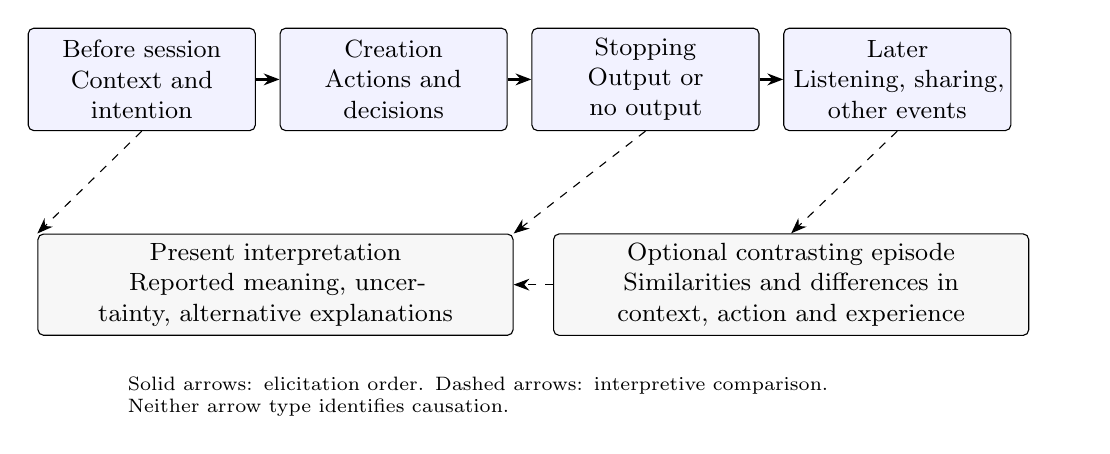
\begin{tikzpicture}[
 phase/.style={draw,rounded corners=2pt,text width=2.65cm,minimum height=1.3cm,align=center,font=\small,fill=blue!5},
 note/.style={draw,rounded corners=2pt,text width=5.8cm,minimum height=1.25cm,align=center,font=\small,fill=black!3},
 arr/.style={-{Stealth[length=2mm]},thick},
 interpret/.style={-{Stealth[length=2mm]},dashed},
 node distance=3mm]
\node[phase] (a) {Before session\\Context and intention};
\node[phase,right=of a] (b) {Creation\\Actions and decisions};
\node[phase,right=of b] (c) {Stopping\\Output or no output};
\node[phase,right=of c] (d) {Later\\Listening, sharing, other events};
\draw[arr] (a)--(b); \draw[arr] (b)--(c); \draw[arr] (c)--(d);
\node[note,below=13mm of b,xshift=-1.5cm] (e) {Present interpretation\\Reported meaning, uncertainty, alternative explanations};
\node[note,right=5mm of e] (f) {Optional contrasting episode\\Similarities and differences in context, action and experience};
\draw[interpret] (a.south) -- (e.north west);
\draw[interpret] (c.south) -- (e.north east);
\draw[interpret] (d.south) -- (f.north);
\draw[interpret] (f.west)--(e.east);
\node[below=4mm of e,anchor=north west,font=\scriptsize,align=left,text width=12cm,xshift=-2cm] {Solid arrows: elicitation order. Dashed arrows: interpretive comparison.\\Neither arrow type identifies causation.};
\end{tikzpicture}

\caption{Prospective elicitation structure. The upper sequence is a recall scaffold, not an assumed causal model; steps may repeat, be absent or occur in another order. The lower boxes distinguish retrospective interpretation and optional contrast. No participant observations are represented.}
\label{fig:episode-elicitation}
\end{figure} The interviewer will separate the original intention from meanings assigned retrospectively, distinguish the session ending from later listening or sharing, and ask about other circumstances that may have contributed to changes. The absence of a reported change is a legitimate account.

A common core guide and documented optional probes permit comparison without requiring identical wording. The interviewer will not show the AIM-ER pathway diagram before open recall. After the pilot, retain the guide version, a brief rationale for revisions, and a record of departures from the common domains. The research team will assess feasibility in terms of interview depth, participant burden and capacity to conduct careful analysis, rather than setting a throughput target that compromises quality.
\subsection{Interview guide}
The table presents an English summary of the interview domains and illustrative prompts. The accompanying Polish guide specifies the wording for fieldwork. Follow-up questions will use the participant's language and ask for examples, counterexamples and clarification without suggesting benefit or harm.

\begin{table}[htbp]
\centering\small
\caption{Interview domains and neutral elicitation prompts.}
\label{tab:interview}
\begin{tabularx}{\linewidth}{@{}p{.23\linewidth}X@{}}
\toprule
Domain & Illustrative prompt \\
\midrule
Context and motive & Think of your latest eligible occasion, including an unfinished attempt. Would you be willing and able to discuss it? If not, we can discuss the next most recent occasion or skip this part. What led to that occasion? Did your intention change as the session progressed? \\
Translation & How did you decide what to put into the prompt, lyrics or musical settings? What did you leave out? \\
Iteration & What happened after the initial attempt, whether or not it produced an output? What led to changes, acceptance or stopping, including stopping without a usable output? \\
Contribution & Which aspects did you regard as your own work, and which as the system's? How did you experience that division and your ability to influence the process? If an artefact exists, to what extent did it feel like yours? What contributed to that perception? \\
Personal meaning & Did the result relate to your personal experience, if at all? How did it relate or fail to relate? Did it match your intentions? What indicated that? If no usable result exists, what significance, if any, did the attempt itself have? \\
Consequences & How do you remember your experience immediately after the session and later? Did anything change? What happened in between? How do you interpret it now? \\
Context and alternatives & How, if at all, did prior musical experience, the tool, other people or alternative ways of creating matter? \\
Contrasting episode & Can you describe another occasion that differed in a meaningful way? What else might explain the difference? \\
Closure & Is there anything important we have not asked? Would you like to withdraw any part of the interview under the agreed procedure? \\
\bottomrule
\end{tabularx}
\end{table}
Probes will distinguish feelings represented in a song from feelings experienced by a participant. The interviewer will not ask whether a presumed mechanism, such as reappraisal, occurred before eliciting the person's account. A participant may describe an episode without specifying the underlying life event. The closing discussion will check whether the participant wishes to take a break or withdraw any material within the agreed withdrawal procedure.


\section{Analysis plan}
\subsection{Preparation and familiarisation}
Audio recordings will be transcribed in Polish, checked against the recording and pseudonymised. Approved note-based interviews will be identified separately; notes will not be treated as verbatim transcripts or used as direct quotations unless an exact quotation was documented under an approved procedure. Assess whether differences in record richness constrain interpretation and report those limitations. Direct identifiers and unnecessarily specific contextual details will be removed or generalised. The corpus of interviews is the unit of thematic analysis. The analyst will read each interview as a whole, annotate uncertainties and develop an episode summary that preserves context and order. The primary and optional contrasting episodes are contextual units of elicitation and interpretation, not independent observations. Discuss the consequences of comfort-related, recall and participation selection; do not infer that the discussed sessions represent all creation attempts. The summary distinguishes the reported goal, action, perceived outcome and interpretation without forcing every account into these categories. Translation into English will occur for reporting, not as the primary analytic corpus.

Before each substantive analytic review, verify corpus eligibility and the current consent and withdrawal status against the approved protected records. Keep an authorised, versioned corpus manifest containing pseudonymous references, record type, inclusion decision and the applicable permission status, without duplicating participant content. Exclude material whose permission is unresolved from analysis until it is resolved. If withdrawal is applicable, follow the approved procedure, remove the affected material from active analytic records, revisit dependent codes, memos, themes and proposed transfers, and document the revision without retaining withdrawn content. A corpus version is a traceability device, not a frozen coding solution; do not assume that an earlier theme remains supported after a corpus change.

\subsection{Reflexive thematic analysis}
Analysis will be recursive \citep{braun2021,byrne2022}. Researchers will record assumptions, prioritise explicit meanings and identify more latent interpretations as their own readings. Coding may overlap and evolve without a predetermined exhaustive codebook. Candidate themes will be checked against extracts and the full corpus, with boundaries revised and exceptions explored. Writing forms part of analysis.

After initial engagement, researchers will explicitly compare themes with AIM-ER, revisiting the corpus where needed. This is a reflexive distinction, not a theory-free first pass. Themes may refine, qualify or challenge the framework, including meanings outside its constructs. Reported sequences do not establish mediation; code frequency does not establish prevalence.

\subsection{Reflexivity and analytic quality}
The research team will document relevant professional and personal backgrounds, assumptions about generative AI, familiarity with music-making and relationships to participants before collection. Researchers will record reflective memos after interviews and at major analytic decisions. Team discussions will challenge alternative interpretations and examine how researcher positions shape the account. They are not designed to measure inter-rater reliability or to produce one objectively correct coding solution. Cohen's kappa, a consensus codebook and numerical saturation thresholds are not quality criteria for the selected reflexive approach. A transparent decision trail will record changes to codes and themes, reasons for revisiting extracts and interpretation of contradictory material. A separate episode memo will record uncertainty in recall, distinctions between reported events and researcher interpretation, and relevant context. A theme-level evidence memo will link supporting extracts to the organising concept and retain divergent cases. These records remain in approved institutional storage; only blank templates and non-identifying methodological descriptions belong in the repository.

We will use the Reflexive Thematic Analysis Reporting Guidelines (RTARG) as the method-specific reporting framework \citep{rtarg2024}, rather than treating COREQ or SRQR \citep{tong2007,obrien2014} as mandatory checklists. Psychology-specific qualitative reporting guidance \citep{levitt2018} provides a complementary account of methodological integrity and situated researcher interpretation. We will explain actual analytic decisions, researcher positioning, the relationship between extracts and interpretive claims, and why procedures presuming a fixed coding truth are inappropriate, rather than certify quality through checklist completion. Participants may correct factual misunderstandings during interviews; they will not be asked to certify a theme as the only valid interpretation. An independent methodological review will assess coherence and reflexivity rather than act as a substitute for analysis.

\subsection{From extracts to an interpretive account}
Preserve extract context and distinguish participant description from researcher interpretation. Each theme memo will specify a central organising concept, relationship to research questions, contextual variation, supporting and contrasting accounts, boundaries and reasons for revisions. A rare account may qualify an interpretation without becoming a theme. Explain why alternative thematic organisations were retained or rejected without voting on a correct solution.

Revisit changing goals, unsuccessful attempts and discrepancies between remembered and current experience without imposing these as themes. Retain uncertainty when a coherent shared pattern is unsupported. Explain how each reported extract supports and limits an interpretive claim; one quotation cannot substantiate a theme or causal mechanism.

\subsection{Link to subsequent research}
Transfer to measurement development requires a specified meaning, boundaries, contexts and contrasting examples. Record the authorised corpus version, theme memo, empirical interpretation or theoretical candidate, proposed indicator or design implication, evidence gaps and retain/revise/defer decision. For example, perceived influence despite limited editing could motivate separate measures of offered control and experienced agency; this is a hypothetical illustration, not a result of P02. Themes need not correspond to reflective latent dimensions; they may motivate formative indicators, prompts or experimental conditions. If no eligible supporting material exists, the transfer remains deferred. Verify approved purpose and disclosure constraints before sharing non-identifying summaries; do not share participant-level records or link cohorts by default. Reassess transfers when themes or permitted material change. Participant quotations require separate disclosure and wording review before item use. Cognitive interviews must evaluate response processes and independent samples must assess psychometric properties. No hypothesis tests, effect sizes or causal estimates are planned; descriptive recruitment counts remain separate from interpretation.

\subsection{Translation and interpretive boundaries}
Analysis will remain in Polish until theme development and selection of illustrative extracts. For English reporting, one bilingual team member will prepare meaning-oriented translations and a second qualified reader will review ambiguous expressions, emotional idioms and culturally specific references. Record substantive interpretive decisions rather than treating translation agreement as a reliability statistic. If no suitable second reader is available, disclose the limitation and retain the original alongside translations within approved storage. Paraphrases introduced to protect confidentiality will not be represented as direct quotations. Separate a participant's attributed explanation from the researcher's thematic interpretation and from a proposed mechanism requiring later testing.

\subsection{Analytic traceability and rival interpretations}
For each research question, retain a trace of relevant contextual material without imposing five corresponding themes. RQ1 addresses reported initial and changing goals; RQ2 addresses decisions and rejected or absent outputs; RQ3 addresses subjective influence, attributed contribution, felt ownership where applicable and personal meaning, including the significance of attempts without an artefact; RQ4 addresses narrated immediate and later experience including no change; RQ5 addresses situated practices and perceived alternatives. Keep absent, not applicable and not elicited distinct: lack of a usable artefact does not imply lack of agency or personal meaning. The final analysis may organise these across questions. The analyst will consider whether apparent emotional change could reflect ordinary listening, time, concurrent events or interpersonal feedback, and whether repeated editing reflects technical constraints rather than perseveration. These are interpretive alternatives, not statistical adjustment variables. Explicitly document where the material does not support a proposed interpretation. Report context-rich illustrative extracts, including contrasting accounts when relevant, without claiming that recurrence counts demonstrate prevalence.

\section{Ethics, data management and dissemination}
The study is prospective and requires institutional ethics review, an approved data-management plan and documented consent before recruitment. The interviewer will not provide psychotherapy, request detailed traumatic disclosures or diagnose participants. If distress occurs, the interviewer will pause, offer the option to skip or terminate, and follow an institutionally approved distress and immediate-risk procedure. Participants will receive relevant support information; confidentiality limits and the escalation procedure must be communicated before consent. If audio recording is declined, proceed only with an institutionally approved note-based option and explicit consent; otherwise do not conduct the interview. Distinguish such records from transcripts and assess their interpretive limitations rather than treating them as verbatim accounts. Confirm a private interview setting where feasible and explain that recordings cannot be fully anonymous. Disable unauthorised cloud recording, automated transcription and meeting assistants. If the connection fails, reconnect only using the agreed contact route; do not resume recording until consent is reconfirmed. Participation and refusal must not affect education, employment or access to services.

Recordings, transcripts and consent records will be stored only in approved institutional storage. No artefact transfer or retention is part of the default protocol. Live showing is optional and unrecorded; disable or pause capture and transcription, avoid copying links or excerpts, and reconfirm consent before resuming. Any exceptional transfer or retention needs a separately approved procedure, consent, rights assessment, defined purpose, access and deletion rules. Separate access-controlled consent and identity records from the pseudonymised analytic corpus. Restrict access to authorised team members; do not upload recordings, verbatim transcripts, personal prompts or artefacts to external generative systems. Do not scrape or analyse creator-community posts under this protocol. Record retention duration, deletion, withdrawal deadlines and access arrangements in the approved information sheet before recruitment. Pseudonymisation is not anonymisation; distinctive stories, lyrics, voices or platform profiles can enable re-identification. Quotations require contextual disclosure review, and potentially identifying material will be omitted or safely paraphrased with clear labelling. Translations will be checked against the source meaning and not presented as verbatim Polish quotations.

Optional artefacts may contain third-party lyrics, voices or personal material. The participant's permission alone does not establish rights for public reproduction. No identifiable audio, lyrics or images will be published without appropriate rights and explicit approval. Findings will be reported using contextualised, de-identified extracts where permitted. Public materials may include the approved interview guide, analysis procedure and non-identifying aggregate summaries; raw data will not be made publicly available. Any future sharing arrangement requires institutional approval and compliance with the consent terms. Before submission, report actual approval identifier, dates, researcher roles, recruitment, deviations, funding, conflicts and author contributions; do not infer them from this protocol.

\section{Discussion: anticipated contribution and limitations}
\subsection{Incremental contribution}
The study may refine or challenge AIM-ER by explaining how personal meaning develops through creative decisions, rather than listing benefits or ownership experiences. Negotiated control alone would extend prior research only if related distinctly to personal meaning or subsequent experience. If the eventual corpus supports only general co-creation processes, report that narrower contribution. Evidence of content relevance from interviews would not establish dimensionality, reliability or construct validity; later survey and AI-MRFS studies require independent evaluation.

\subsection{Discriminating interpretations}
Interviews cannot separate effects of AI from writing, listening, time or concurrent activities. Contrasting episodes may clarify interpretations but cannot establish controlled within-person effects. Technical novelty without emotional change is as relevant as perceived relief.

\subsection{Implications for subsequent research}
Accounts linking perceived influence to personally meaningful outputs could motivate experiments varying revision opportunities; accounts locating meaning in lyrics could motivate comparisons with writing alone or existing music. Neither example constitutes a result or a prediction confirmed by P02. Prospective outcome definitions and appropriate baseline assessments would be required. Immediate relief alongside later distress would motivate distinct measurement times. Unsupported AI-specific mechanisms should be narrowed or deferred.

\subsection{Limitations and transferability}
Retrospective interviews depend on memory, narrative reconstruction and willingness to disclose. Accounts may emphasise successful outputs or socially legitimate reasons for creation. Recruitment through online communities may privilege engaged users. Interviews in Polish cannot establish cultural universality, and rapidly changing platforms constrain transferability across model versions. Voluntary artefacts are selectively available and are not an independent validation sample. Interviews conducted without audio recordings may provide less detailed material than transcribed interviews; the consequences of this difference for particular interpretations will be examined rather than assuming equivalent records. The recall window and the requirement that an episode be discussable may underrepresent people who stopped using generators earlier or decline to describe distressing experiences. The interviewer and participants may also share assumptions about the value or risks of AI, making reflexive consideration of the interview interaction essential. These limitations affect the scope of interpretive claims and cannot be eliminated by increasing the sample alone. No claims about frequencies, clinical benefit, neural mechanisms or causal mediation will follow from the themes. Subsequent longitudinal and experimental studies would be required to test the timing and causal implications of proposed mechanisms. The final empirical article will report only findings supported by collected and ethically usable material; this protocol contains no results. Transferability will be considered through contextual description of the recruitment channels, platform affordances, participants' experience and the circumstances of the accounts, without identifying individuals or treating diversity as population representativeness.

\section{Conclusion}
This protocol proposes an episode-centred, contextualist qualitative investigation of AI-assisted music creation. Its contribution will depend on interpretive depth, attention to divergent experiences and a coherent account of how emotional meaning is attributed to creative practices. The study can inform theory and future measurement but cannot establish efficacy, prevalence or causal mechanisms.
\section{Additional qualitative research domains}
The episode-centred guide will include optional follow-up prompts about the transition from lived experience to a musical representation: identifying or borrowing emotional labels, use of metaphor, changes in the narrative during revision, recognition of one's intended meaning, and the difference between first-person immersion and an observer perspective. Ask whether participants experienced insight, tension release, a sense of closure, pride, aesthetic pleasure or absorption, and whether such experiences persisted, changed or disappeared after later listening. Invite accounts of unchanged or worsened affect and of attempts that did not produce a usable artefact. Terms such as catharsis and self-therapy will be explored as participants' own interpretations rather than suggested benefits or clinical categories.

Ask about private creation, selective sharing and public posting, anticipated judgement, perceived anonymity, belonging, acceptance, rejection and unwanted disclosure. Explore whether creative activity facilitated subsequent communication or displaced it, and how participants decided to continue, revise, stop or switch strategies. Contrast repetitive listening or generation that felt purposeful with episodes described as difficult to disengage from. Where voluntarily offered, a participant may describe or privately present an artefact under the existing consent procedure; this is a recall aid, not independent evidence of prior affect. Do not elicit traumatic detail, assume positive effects, or infer a diagnosis from a song. Use these domains as sensitising prompts after free recall rather than a fixed coding scheme. The resulting interpretations may inform P03 and item content in P05, but do not validate scale structure or causal mechanisms.

\subsection{Candidate probes for contrasting episodes}
To operationalise the expanded interview scope, the following neutral probes supplement rather than replace the approved episode guide: What did you want to achieve before you started? Which decisions did you make yourself, and which did you delegate? Did the words or music represent something you already understood, or did they help you notice something new? Did the experience look different after listening, and if so, how? What happened when you returned to the song later? If another person heard the result, how did you interpret their response? What made you decide to stop or continue? Ask for counterexamples and experiences without any change, rather than eliciting agreement with a putative therapeutic mechanism.

Contrast a private episode with a shared episode only when the participant has such experiences and wishes to discuss them. A report of relief accompanied by postponed action is not contradictory; explore how both meanings coexist in the account. The differentiation of adaptive and maladaptive musical engagement in \citet{carlson2015} and the regulatory flexibility account of \citet{bonanno2013} inform attention to such contrasts, without imposing diagnostic categories. The analysis will use reflexive thematic interpretation \citep{braun2021}; a thematic matrix may organise cases by context and contrasting meanings but is not a frequency estimate or a reliability test of a predetermined set of mechanisms. The expanded prompts remain candidate guide revisions pending pilot and ethics review.

\subsection{Relatedness, disclosure and the social setting of creation}
Music-related bonding has been discussed in relation to shared rhythmic action and synchrony \citep{tarr2014}. A person posting a generated song may instead seek recognition, communicate a private experience or participate in a community without performing music jointly. The interview should distinguish a felt connection during creation, imagined communication to a particular audience, actual sharing and the meaning attributed to later responses. Ask whether the community context changed the willingness to create or disclose and whether the same artefact would have been made in private. Include neutral, unwelcome and absent feedback without assuming that public disclosure is beneficial. These accounts can refine hypotheses about social functions but cannot establish effects of synchrony, social validation or changes in loneliness.

\printbibliography
\end{document}
